\chapter{Implementacja programu}
W rozdziale piątym zostały przedstawione najważniejsze fragmenty sposobu implementacji programu. 

\section{Realizacja detekcji pięciolinii}

Detekcja pięciolinii została opracowana na podstawie pracy M. Szwocha \textit{A Robust Detector for Distorted Music Staves}.

Jedną z najbardziej przydanych właściwości pięciolinii jest ich forma, mianowicie pięć prostych, równoodległych linii, co czyni je perfekcyjnymi kandydatami do detekcji zniekształceń wprowadzonych przez proces fotografowania, pozwalając na usunięcie niedoskonałości geometrycznych obrazu.

Proces detekcji pozycji pięciolinii na obrazie został zrealizowany przy pomocy analizy histogramów okienek próbnikowych. Okienkiem próbnikowym nazywany jest fragment obrazu rozciągający się na całą jego wysokość i pewną szerokość, przy pomocy którego dokonywana jest analiza obrazu, poprzez analizę jego mniejszych fragmentów. Po analizie okienka na danej części obrazu, jego pozycja jest przesuwana o daną odległość w osi poziomej, po czym następuje analiza następnego wycinka. Poszczególne okienka próbnikowe nie mają na siebie bezpośredniego wpływu podczas analizy.

\begin{figure}[H]
	\centering
	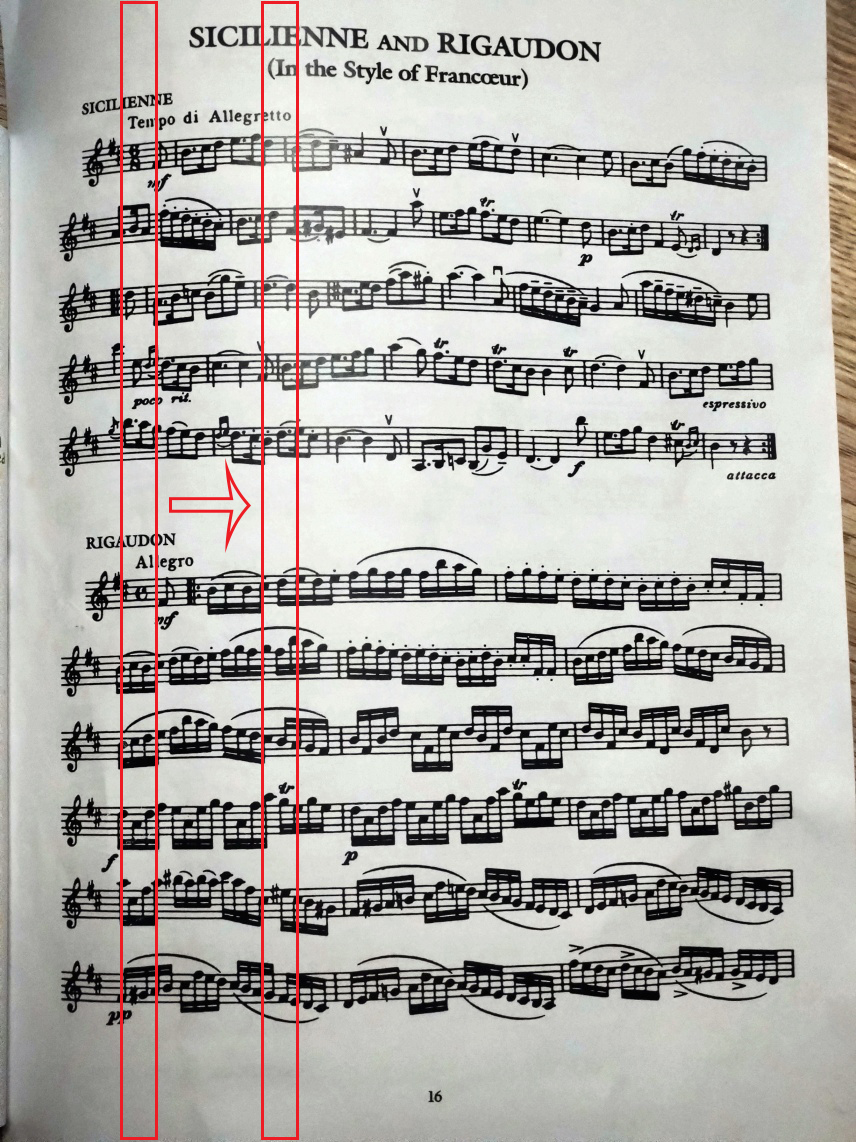
\includegraphics[width=12cm]{images/probe window demo.jpg}
	\caption{Wizualizacja okienka próbnikowego na zdjęciu nut.}
	\label{fig:probe_window_demo}
\end{figure}

\pagebreak

\subsection{Realizacja detekcji pozycji wypaczonych pięciolinii na obrazie}

\begin{lstlisting}[caption={\pyth|find_staves_points()| - funkcja odnajdywania pozycji pięciolinii na obrazie}, label={find-staves-points}, language=Python]
def find_staves_points(img, img_name, stride = 2):
	img = enhance_image(img, img_name)
	
	img_y, img_x = img.shape[:2]
	
	staff_line_dist = find_staff_line_distance(img)
	if staff_line_dist == -1:
		return -1, 0
	
	staves_positions = find_staves_positions(staff_line_dist, stride, img)
	if len(staves_positions) == 0:
		return -1, -1
	else:
		staves_points_list = make_staves_points_list(staves_positions, staff_line_dist)
		if staves_points_list == -1  or len(staves_points_list) == 0:
			return -1, -1

	return staves_points_list, staff_line_dist
\end{lstlisting}

Powyższa funkcja \pyth|texfind_staves_points()| jest odpowiedzialna za znalezienie i stworzenie listy punktów, które definiują pozycję pięciolinii. Funkcja ta przyjmuje za argumenty wczytany obraz, jego nazwę oraz liczbę kroków. Natomiast zwraca listę zawierającą punkty opisujące położenie pięciolinii oraz odległość między liniami pięciolinii, albo wartości zawiadamiające kod wywołujący tę funkcję o wystąpieniu błędu.

Pierwszym krokiem do poprawnej detekcji pięciolinii na obrazie jest uwydatnienie pożądanych jego cech, co jest wykonywane przy pomocy funkcji \pyth|enchance_image()|, dzięki której możliwa jest łatwiejsza analiza badanego obrazu. Następnie następuje wywołanie funkcji odpowiedzialnej za odnalezienie odległości pomiędzy liniami pięciolinii \pyth|find_staff_line_distance()|, poprzez przekazanie obrazu. Jeśli tejże funkcji udało się poprawie odnaleźć szukaną wartość, następuje wywołanie kodu mającego odszukać pozycje pięciolinii na obrazie \pyth|find_staves_positions()| przez przekazanie odnalezionej wcześniej odległości, liczby kroków oraz obrazu. Kiedy operacja się powiedzie, następuje reformatowanie listy uzyskanych punktów przez funkcję \pyth|make_staves_points_list()|, by punkty zawarte w jednej liście zawierały pozycje pojedynczej pięciolinii. Operacja ta jest potrzebna, gdyż uzyskane wartości są ułożone w listach reprezentujących pozycje w pionowych wycinkach, gdzie następna część programu będzie potrzebowała ich w formacie punktów pojedynczej pięciolinii na jedna listę. W wypadku powodzenia wszystkich operacji następuje zwrot listy pozycji oraz odległości pomiędzy liniami pięciolinii.



\subsubsection{Realizacja uwydatniania obrazu} \label{enhance_image_impl}

\begin{lstlisting} [caption={\pyth|enhance_image()| - funkcja uwydatniania obrazu.}, label={enhance-image}, language=Python]
	def enhance_image(img):
	if len(img.shape) == 3:
		img = cv2.cvtColor(img, cv2.COLOR_RGB2GRAY)
	
	img = cv2.GaussianBlur(img, (5, 5), 0)
	img = cv2.adaptiveThreshold(img, 255, cv2.ADAPTIVE_THRESH_MEAN_C, cv2.THRESH_BINARY, 55, 7)
	
	return img
\end{lstlisting}

Znajdująca się powyżej funkcja ma za zadanie zmodyfikowanie obrazu, by ten nadawał się do jego analizy. Odbywa się to przez konwersję obrazu do odcieni szarości, jeśli jest on obrazem kolorowym, po czym następuje seria modyfikacji, pozwalających na uwydatnienie pożądanych informacji z obrazu.

Pierwszą modyfikacją jest rozmycie gaussowskie, dzięki któremu z obrazu usuwana jest część szumu oraz drobne niedoskonałości są rozmywane, by w następnym kroku możliwe było lepsze określenie wartości znajdujących się ponad progiem. Kolejną modyfikacją zastosowaną na obrazie jest progowanie adaptacyjne, które w przeciwieństwie do zwykłego progowania, pozwala na usunięcie cieni z obrazu, zachowując znajdujące się w nich dane, które mogą być potrzebne do poprawnej analizy. Jednocześnie progowanie adaptacyjne automatycznie znajduje odpowiednie wartości progu, dzięki czemu nie istnieje potrzeba określania go ręcznie, co wymaga znaczącej ilości czasu i prób, by znaleźć taką wartość, która będzie działała w jak najszerszym zakresie danych wejściowych. Ostatnią modyfikacją dotykającą obraz jest erozja, która służy do usunięcia niechcianych punktów i wyostrzenie linii znajdujących się na obrazie, co jest wymagane dla poprawnego odszukiwania pięciolinii.



\subsubsection{Realizacja odnajdywania odległości między liniami pięciolinii} \label{find_staff_line_distance_impl}

\begin{lstlisting} [caption={ \pyth|find_staff_line_distance()| - funkcja odnajdywania odległości między liniami pięciolinii.}, label={find-staff-line-distance}, language=Python]
def find_staff_line_distance(img = np.array):
	img_y, img_x = img.shape[:2]
	probe_window_size = img_x // 40
	probe_window_start_idx = img_x // 5
	probe_window_end_idx = img_x - probe_window_start_idx
	probe_window_hist_arr = np.zeros(img_y)
	staff_line_distance_list = []
	
	for i in range(probe_window_start_idx, probe_window_end_idx, probe_window_size*6):
		make_histogram_array(i, img_y, probe_window_size, img, probe_window_hist_arr)
		peaks_list = filter_out_peaks(probe_window_size, probe_window_hist_arr)
		staff_line_distance = find_staff_line_distance_in_probe(peaks_list)
		
		if staff_line_distance != 0:
			staff_line_distance_list.append(staff_line_distance)
		
		probe_window_hist_arr = np.zeros(img_y)
	
	if len(staff_line_distance_list) != 0:
		return sum(staff_line_distance_list) // len(staff_line_distance_list)
	else:
		return -1
\end{lstlisting}

Umieszczony powyżej kod funkcji \pyth|find_staff_line_distance()| odpowiedzialny jest za odnalezienie odległości pomiędzy liniami pięciolinii na zdjęciu zapisu nutowego. Funkcja ta zaczyna pracę poprzez inicjalizację niezbędnych zmiennych zawierających wartości takie jak: rozmiary obrazu, rozmiar okienka próbnikowego, indeks początkowy poszukiwania, indeks końcowy, tablicę na której będą przechowywane wartości odczytane z okienka próbnikowego, oraz lista potencjalnych odległości z okienek próbnikowych.

Wartości tych zmiennych nie są przypadkowe, szerokość okienka została dobrana eksperymentalnie, podczas to których eksperymentów stwierdzono, iż wielkość równa jednej czterdziestej szerokości obrazu daje zadowalające rezultaty, dające poprawne wielkości, natomiast pozycja początkowa i końcowa okienka próbnikowego gwarantuje, na poprawnie wykonanych zdjęciach, znajdowanie się pięciolinii w badanym zakresie.

Właściwe odszukiwanie odbywa się iteratywnie poprzez przesuwanie okienka próbnikowego o wielkości większe od jego szerokości, gdyż nie potrzebujemy analizować całego obrazu, tylko kilka jego fragmentów. Analizowanie pojedynczego okienka może dać niepoprawną wartość odległości, zatem obraz jest analizowany w kilku miejscach, by pozyskać właściwą miarę.

W każdym kroku pętli tworzona jest tablica, na podstawie której powstaje histogram okienka, dzięki funkcji \pyth|make_histogram_array()|, która zlicza wystąpienia ciemnych pikseli w  każdym rzędzie badanego okienka. Następnie z uzyskanej tablicy, w funkcji \pyth|filter_out_peaks|, odfiltrowywane są indeksy wysokich wartości histogramu, które powinny być liniami rozpinającymi się na większość szerokości okienka. Na podstawie uzyskanej listy indeksów w funkcji \pyth|find_staff_line_distance()| odszukiwana jest odległość między liniami pięciolinii, dzięki własności zapisu nutowego, w którym najczęściej występującą odległością między dwiema liniami w osi pionowej jest właśnie odległość pomiędzy składowymi pięciolinii. Jeśli odnaleziona wartość nie jest zerem, to jest dodawana do listy potencjalnych odległości. Przed przejściem do następnego kroku pętli, tablica okienka próbnikowego jest zerowana, by poprzednia analiza nie wpływała na analizę kolejnego okienka.

Gdy analiza okienek się zakończy, jeśli lista potencjalnych odległości nie jest pusta, zwracana jest średnia arytmetyczna z listy odległości w formie wartości całkowitej, natomiast jeśli lista jest pusta, zwracana jest wartość \textit{-1}, by poinformować kod wywołujący o błędzie operacji.



\subsubsection{Realizacja odnajdywania pozycji pięciolinii}

\begin{lstlisting}[caption={\pyth|find_staves_positions()| - funkcja odnajdywania pozycji pięciolinii.}, label={find-staves-positions}, language=Python]
def find_staves_positions(staff_line_distance, stride = 1, img = np.array):
	img_y, img_x = img.shape[:2]
	probe_window_size = (staff_line_distance * 2) + 5
	probe_window_start_idx = probe_window_size * 2
	probe_window_end_idx = img_x - probe_window_start_idx
	probe_window_hist_arr = np.zeros(img_y)
	staves_positions_list = []
	
	for i in range(probe_window_start_idx, probe_window_end_idx, probe_window_size * stride):
		make_histogram_array(i, img_y, probe_window_size, img, probe_window_hist_arr)
		peaks_list = filter_out_peaks(probe_window_size, probe_window_hist_arr)
		staves_positions = get_staves_positions(i, staff_line_distance, peaks_list)
		staves_positions_list.append(staves_positions)
		
		probe_window_hist_arr = np.zeros(img_y)
	
	if len(staves_positions_list) == 0:
		return -1
	else:
		return staves_positions_list
\end{lstlisting}

Odszukiwanie pozycji pięciolinii, realizowane w funkcji \pyth|find_staves_positions()| odbywa się analogicznie do działania \pyth|find_staff_line_distance|, z pewnymi różnicami, mianowicie:
\begin{itemize}
	\item szerokość okienka próbnikowego wynosi dwukrotność odległości między liniami pięciolinii, plus pięć pikseli. Wynika to z właściwości zapisu nutowego, gdzie główka nuty jest nieco szersza, niż odległość między liniami, przez co taka wartość zapewnia, że główka nuty nie będzie zajmowała całej szerokości badanej części obrazu, zaburzając odczytywane dane, scalając ze sobą dwie linie.
	\item początkowa pozycja jest ustalona na dwie szerokości okienka od lewej krawędzi, końcowa zaś na dwie szerokości od prawej krawędzi, by uniknąć niepotrzebnej analizy granic obrazu, na których zazwyczaj nic się nie znajduje, lub znajdują się tam losowe wartości uzyskane z tła.
	\item szerokość kroku jest uzależniona od szerokości okienka oraz przekazanej wartości kroku, która mówi o ile okienko ma się przesuwać w każdym kroku pętli.
	\item po odnalezieniu indeksów dużych wartości histogramu w każdym korku pętli, wywoływana jest funkcja \pyth|get_staves_postitions|, która szuka sekwencji, odległych od siebie o wcześniej odszukaną odległość pięciu indeksów na całej wysokości okienka, tworząc listę punktów z danego wycinka, na którym znajdują się pięciolinie. Zwrócona lista jest dodawana do listy pozycji na których zostały wykryte pięciolinie, po czym resetowana jest tablica okienka próbnikowego.
\end{itemize}


Gdy analiza okienek się zakończy, jeśli lista pozycji nie jest pusta, to jest ona zwracana, natomiast jeśli lista jest pusta, zwraca się wartość \textit{-1}, by poinformować kod wywołujący o błędzie operacji.

\section{Usuwanie wypaczania obrazu}

\section{Segmentacja obrazu}

\section{Model głębokiego uczenia do rozpoznawania zapisu nutowego}

